This chapter covers the theory of the most widely used method for point forecasting in the EF literature. Besides discussing the theory underlying these models, this and the following chapter include also a couple of worked examples in order to get acquainted with the practical applications of models.


% \section{Exponential smoothing}
% Exponential smoothing was developed by Brown \cite{brown1959statistical}, Holt \cite{holt1957forecasting}, Winters \cite{winters1960forecasting}.
% The idea is to forecast future values by taking a weighted average of past observations, where weights decay exponentially in time.
% \begin{equation}
%     \begin{aligned}
%         \hat{y}_{t+h|t}=& l_{t}+hb_{t}+s_{t+h-m(k+1)}
%         \\
%         l_t=&\alpha (y_t-s_{t-m})+(1-\alpha)(l_{t-1}+b_{t-1})
%         \\
%         b_t=& \beta(l_t-l_{t-1})+(1-\beta)b_{t-1}
%         \\
%         s_t=&\gamma(y_t-l_{t-1}-b_{t-1})+(1-\gamma)s_{t-m}
%     \end{aligned}
% \end{equation}
% where $0\leq \alpha \leq 1$ is the smoothing parameter and k is the integer part of $\frac{(h-1)}{m}$.%that is k encodes seasonalities
% Optimal parameters are obtained by minimising the sum of squared errors.


\section{Multiple linear regression}

\section{Autoregressive models}
explain their theory
and how the procedure how they are used
IMPORTANT: load series is not a stationary series so before applying AR we have to perform stationary tests or differencing steps
\subsection{ARIMA}
\subsection{ARIMAX}
\subsection{SARIMA}
\subsection{SARIMAX}

\section{Generalized additive model}
%prophet meta
\section{K-nearest neighbors}

\section{Support vector regression}
Developed at the AT\&T Bell Laboratories by Vapnik et al. \cite{cortes1995support}, \cite{vapnik1997support}, support vector machines SVMs are one of the most popular techniques within the field of statistical learning.
\\
The goal of support vector regression is finding a function f(x) with at most $\epsilon$ deviation from the actual observed data $y_i$ $\forall i$ and as flat as possible. 
Put differently, we would like a model to keep error less than the $\epsilon$ threshold,  
%https://stats.stackexchange.com/questions/5945/understanding-svm-regression-objective-function-and-flatness
In standard SVR we have
\begin{equation}
    f(x)=\langle w,x \rangle +b \ \textrm{with} \ w \in X, b \in R
\end{equation}
Where $X$ denotes the space of the input patters $x_i$.
We can translate the flatness requirement into minimising the squared norm of w. Doing so we can formulate our problem as a convex optimisation problem.
\begin{equation}
    \begin{aligned}
        \min \quad& \frac{1}{2}\|w\|^2
        \\
        s.t. \quad& y_i-\langle w, x_i\rangle-b\leq \epsilon
        \\
        \quad& \langle w, x_i\rangle +b-y_i\leq \epsilon
    \end{aligned}
\end{equation}
Next, we need to introduce the slack variables $\xi$ and $\xi^*$, in order to handle the above formulate optimisation problem.
We obtain the following formulation
\begin{equation}
    \begin{aligned}
        \min \quad& \frac{1}{2}\|w\|^2+C\sum\limits_{i=1}^l(\xi_i+\xi_i^*)
        \\
        s.t. \quad& y_i-\langle w, x_i\rangle-b\leq \epsilon+\xi
        \\
        \quad& \langle w, x_i\rangle +b-y_i\leq \epsilon+\xi^*
        \\
        \quad& \xi_i\geq0
        \\
        \quad& \xi_i^*\geq0
    \end{aligned}
\end{equation}
The C constant trades off between $\epsilon$ deviation tolerance and flatness of the function f.
We seek to minimise the epsilon insensitive loss function, defined as follows
\begin{equation}
    \|\xi\|_\epsilon:=\begin{cases}
        0 \quad& \textrm{if} \ \|\xi\|\leq \epsilon
        \\
        \|\xi\|-\epsilon \quad& \textrm{if} \ \|\xi\|\leq \epsilon
    \end{cases}
\end{equation}
The model is depicted in figure \ref{fig:svm_simple}. The gry band is called the epsilon insensitive tube, only the points outside it are accounted by the loss function.
\begin{figure}
    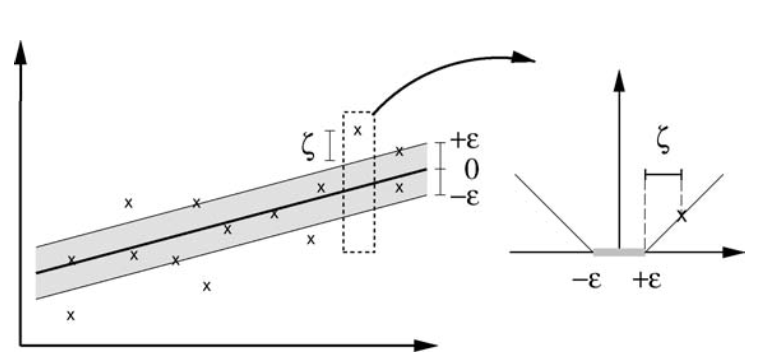
\includegraphics[width=\textwidth]{images/svm_simple.png}    
    \caption{Support vector regression,\cite{learning_with_kernels}}
    \label{fig:svm_simple}
\end{figure}
Smola et al. \cite{smola2004tutorial} point out that considering the dual formulation makes our optimisation problem easier to solve. Doing so we have
\begin{equation}
    \begin{aligned}
        \max \quad& -\frac{1}{2}\sum\limits_{i,j=1}^l(\alpha_i-\alpha_i^*)(\alpha_j-\alpha_j^*)\langle x_i,x_j\rangle +\sum\limits_{i=1}^l(\alpha_i-\alpha_i^*)(y_i-\epsilon)
        \\
        s.t. \quad& \sum\limits_i=1^l(\alpha_i-\alpha_i^*)=0
        \\
        \quad& \alpha_i, \alpha_i^* \in [0, C]
    \end{aligned}
\end{equation}
Rearranging the gradient of the lagrangian with respect to w, we obtain the so called support vector expansion.
\begin{equation}\label{eq:support vector expansion}
    w=\sum\limits_{i=1}^l(\alpha_i-\alpha_i^*)x_i
\end{equation}
That means that w can be completely described as a linear combination of the training features $x_i$.
Notice, the complexity of the function representation is independent of the feature space dimensionaly but depends only on the number of support vectors; that is those point $i$ for which $(\alpha_i-\alpha_i^*)\neq 0$
Notice that, we do not needd to compute w explicitly in order to evaluate f(x).
Furthermore, equation \ref{eq:support vector expansion} implies
\begin{equation}
    f(x)=\sum\limits_{i=1}^l(\alpha_i-\alpha_i^*)\langle x_i, x\rangle +b
\end{equation}
Employ the Karush-Kuhn-Tucker conditions, b can be retrieved easily. Particularly, use the condition that the product between the constraints and the dual variable has to vanish. These implies that the lagrange multipliers $\alpha_i, \alpha_i^*$ may be nonzero only for the samples inside the epsilon insensitive tube. Consequently for any of these data points, the equality $b=y_i-\langle w, x_i-\epsilon\rangle$ holds.
To get an idea, see figure \ref{fig:svr1} for a how support vector regression handles a sinusoidal function with noise.
\\
\begin{figure}
    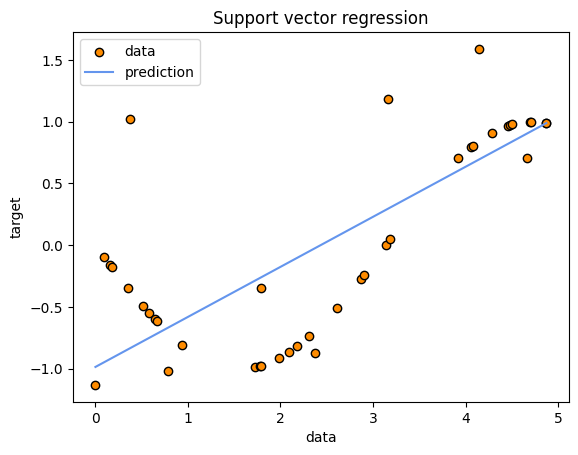
\includegraphics[width=\textwidth]{images/svr1.png}
    \caption{support vector regression}
    \label{fig:svr1}
\end{figure}

\section{Artificial neural networks}
\subsection{DNN}
\subsection{LSTM}
\subsection{DeepAr}
\subsection{AR Net}

\section{Kernel methods}
\subsection{Kernel regression}
\subsection{Kernel support vector regression}
Support vector regression can be kernelized by swapping the R2 euclidean dot product of data x with the dot product in the higher feature space F. Doing so, the optimisation problem can be restated as
\begin{equation}
    \begin{aligned}
        \max \quad& -\frac{1}{2}\sum\limits_{i,j=1}^l(\alpha_i-\alpha_i^*)(\alpha_i-\alpha_i^*)k(x_i, x_j)+\sum\limits_{i=1}^l(y_i-\epsilon)(\alpha_i-\alpha_i^*)
        \\
        s.t. \quad& \sum\limits_{i=1}^l(\alpha_i-\alpha_i^*)=0
        \\
        \quad& \alpha_i, \alpha_i^* \in [0,C]
    \end{aligned}
\end{equation}
Our regressor f is then given by
\begin{equation}
    \begin{aligned}
        \sum\limits_{i=1}^l(\alpha_i-\alpha_i^*)k(x_i, x)+b
    \end{aligned}
\end{equation}
Notice, in this setting w is no longer given explicitly and we seek for the flattest function in the feature space not the input space.
See figure \ref{fig:svr2} and figure \ref{fig:svr3} for two examples. In the former we have used a polynomial kernel while in the latter the standard radial basis function kernel.
\begin{figure}
    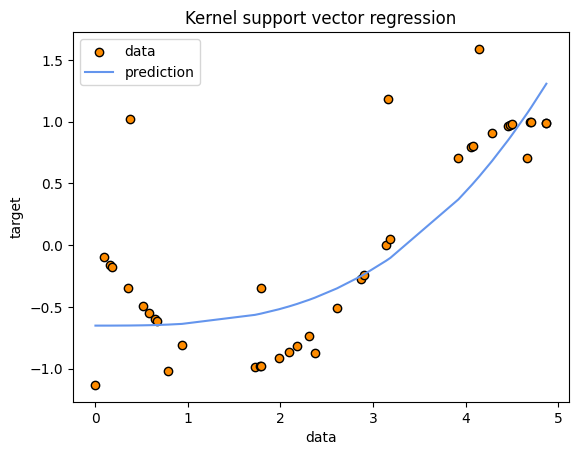
\includegraphics[width=\textwidth]{images/svr2.png}
    \caption{polynomial support vector regression}
    \label{fig:svr2}
\end{figure}

\begin{figure}
    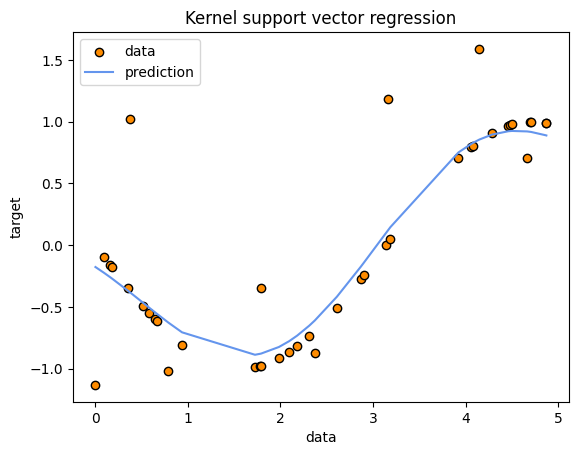
\includegraphics[width=\textwidth]{images/svr3.png}
    \caption{rbf support vector regression}
    \label{fig:svr3}
\end{figure}
Comparing theese pictures with figure \ref{fig:svr1}, it can be concluded that introducing kernels allows support vector regression to handle non linearities in the data.